\iffalse
\begin{frame}{Analyse des mouvements}
        Les données doivent être analysées, soit par un expert, soit par le système

        \begin{block}{Analyse empirique}
            Pas de formalisation des caractéristiques du geste, différences morphologiques, expertise difficile à formaliser (domaine médical)
        \end{block}
        
        \begin{block}{Analyse automatique}
            Connaissance experte formalisable et quantifiable
        \end{block}
     \end{frame}

    \subsection{EIAH pour le mouvement}
    \begin{frame}{\subsecname}
        Plusieurs méthodes et objectifs pour les EIAH dédiés au mouvement :
        \begin{itemize}[label=$\bullet$]
            \item Affichage du mouvement à reproduire \mycite{Kora20151559}
            \item Manipulation d'objets \mycite{Chellali2016Aia}
            \item Immersion en réalité virtuelle (EVAH) \mycite{Baldominos2015AAt}
            \item Ludification \mycite{Alankus2010TCG}
        \end{itemize}

        \vspace{1cm}
    \end{frame}
    
    \subsection{Limites des systèmes existants}
    \begin{frame}{\subsecname}
        Les EIAH dédiés à l'apprentissage du mouvement présentent souvent une ou plusieurs limites :
        \begin{block}{Limites généralistes}
            \begin{itemize}[label=$\bullet$]
                \item Conception \textit{ad-hoc}
                \item Intégration de la connaissance experte difficile sans ré-ingénierie conséquente
            \end{itemize}
        \end{block}
        
        \begin{block}{Limites de l'analyse automatique}
            \begin{itemize}[label=$\bullet$]
                \item Problème de la taille du corpus d'apprentissage
                \item Reconstitution d'un autre corpus pour un autre domaine applicatif
                \item Expert écarté du processus d'apprentissage
            \end{itemize}
        \end{block}
    \end{frame}
    
    \section{Matériels de capture}
    \begin{frame}{Représentation informatique du mouvement}
        \centering
        \resizebox{!}{4cm}{%
        \begin{tikzpicture}
            \node[draw, rounded corners=3pt, align=center] (chest) at (0,-1.5) {chest};
            \node[draw, rounded corners=3pt, align=center] (neck) at (0,0) {neck};
            \node[draw, rounded corners=3pt, align=center] (head) at (0,1) {head};
            \node[draw, rounded corners=3pt, align=center] (leftshoulder) at (-2,0) {l. shoulder};
            \node[draw, rounded corners=3pt, align=center] (rightshoulder) at (2,0) {r. shoulder};
            \node[draw, rounded corners=3pt, align=center] (lefthand) at (-2,-1) {l. hand};
            \node[draw, rounded corners=3pt, align=center] (righthand) at (2,-1) {r. hand};
            \node[draw, rounded corners=3pt, align=center] (hips) at (0,-3) {hips (ROOT)};
            \node[draw, rounded corners=3pt, align=center] (leftknee) at (-2,-4) {l. knee};
            \node[draw, rounded corners=3pt, align=center] (rightknee) at (2,-4) {r. knee};
            \node[draw, rounded corners=3pt, align=center] (leftfoot) at (-2,-5) {l. foot};
            \node[draw, rounded corners=3pt, align=center] (rightfoot) at (2,-5) {r. foot};

            \node[] (hips_offset) at (-4,-3) {

            $\begin{array}{ccc}
                x & y & z \\
               (0 & 0 & 0) \\
            \end{array}$

            };


            \node[] (chest_offset) at (-4,-1.5) {

            $\begin{array}{ccc}
                x & y & z \\
               (0 & 1 & 0) \\
            \end{array}$

            };

            \node[draw] (c_base) at (-7,-2) {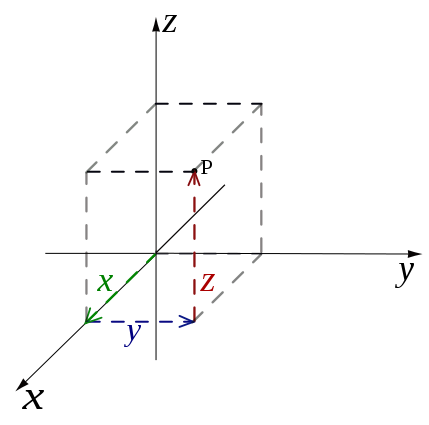
\includegraphics[scale=0.2]{img/coordinates.png}};



            \node[] (hips_orientation) at (4,-3) {

            $\begin{array}{ccc}
                \alpha & \beta & \gamma \\
                (45 & 0 & 45) \\
            \end{array}$

            };


            \node[] (chest_orientation) at (4,-1.5) {

            $\begin{array}{ccc}
                \alpha & \beta & \gamma \\
                (78 & 10 & 21) \\
            \end{array}$

            };

            \node[draw] (c_base) at (-7,-2) {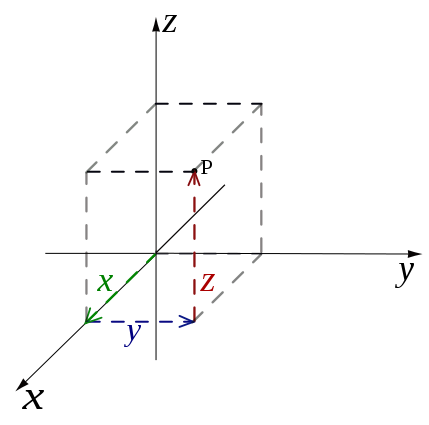
\includegraphics[scale=0.2]{img/coordinates.png}};

            \node[draw] (c_base) at (7,-2) {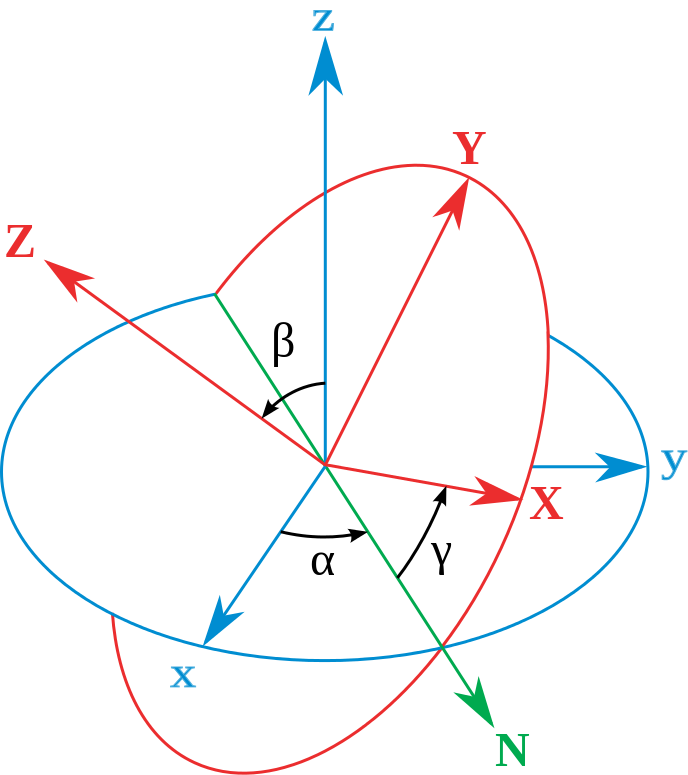
\includegraphics[scale=0.1]{img/euler_angles.png}};


            \draw(hips) -- (chest);
            \draw(chest) -- (neck);
            \draw(neck) -- (head);
            \draw(neck) -- (leftshoulder);
            \draw(leftshoulder) -- (lefthand);
            \draw(neck) -- (rightshoulder);
            \draw(rightshoulder) -- (righthand);
            \draw(hips) -- (leftknee);
            \draw(leftknee) -- (leftfoot);
            \draw(hips) -- (rightknee);
            \draw(rightknee) -- (rightfoot);

            \draw[loosely dotted, ->] (hips) -- (hips_offset);
            \draw[loosely dotted, ->] (chest) -- (chest_offset);

            \draw[loosely dotted, ->] (hips) -- (hips_orientation);
            \draw[loosely dotted, ->] (chest) -- (chest_orientation);
        \end{tikzpicture}
        }
    \end{frame}
    
    \subsection{Objectifs et coûts}
    \begin{frame}{Dispositifs de captation}
        Plusieurs objectifs possibles pour l'apprentissage du geste :
        \begin{itemize}[label=$\bullet$]
            \item Le mouvement est la finalité de l'apprentissage
            \item La manipulation d'un objet est la finalité de l'apprentissage 
        \end{itemize}
        
        Les dispositifs de captures ne sont pas les mêmes en fonction des objectifs et des contraintes :
        \begin{itemize}[label=$\bullet$]
            \item Objet de la captation
            \item Coût
            \item Qualité des données
            \item Encombrement
            \item Espace disponible
            \item Chaîne de traitement des données nécessaire
            \item Retours sensoriels ou visuels souhaités
        \end{itemize}
    \end{frame}
    
    \subsection{Caméra RGB}
    \begin{frame}{\subsecname}
        \begin{block}{Caméra RGB}
            \begin{itemize}[label=$\bullet$]
                \item Captation d'une vidéo
                \item Détermination d'un squelette à partir de la vidéo
            \end{itemize}
            Plusieurs méthodes d'extraction possible \mycite{Sarafianos2016DHp} : projection d'un squelette 3D en 2D pour obtenir une correspondance, utilisation de contraintes rigides sur plusieurs images successives, etc.\\
            Possibilité d'utiliser une vidéo stéréo pour reconstituer le squelette 3D \mycite{Liu2016Tb3}
        \end{block}
    \end{frame}
    
    \subsection{Caméra RGB-D}
    \begin{frame}{\subsecname}
        \begin{block}{Caméra RGB-D}
            \begin{itemize}[label=$\bullet$]
                \item Captation d'une vidéo + une carte de profondeur
                \item Pas d'inférence à partir d'une image 2D seulement
                \item Problème d'occlusion (possibilité d'utiliser plusieurs caméras synchronisées \mycite{Regazzoni2014Rcv}, mais nécessite un emplacement de capture dédié)
            \end{itemize}
            Sport \mycite{YAMAOKA2013912, Yoshinaga2015Doa, Kora20151559}, 
        \end{block}
    
    \end{frame}
    
    \subsection{Caméras infrarouge}
    \begin{frame}{\subsecname}
        \begin{block}{Caméras infrarouge}
            \begin{itemize}[label=$\bullet$]
                \item Meilleur précision
                \item Plusieurs captures possibles en simultané \mycite{Pfister2014Cao, Yang2016HUL}
                \item Coût très élevé
                \item Nécessite un environnement de capture dédié
                \item Chaîne de traitement lourde
            \end{itemize}
        \end{block}
    \end{frame}
    
    \subsection{Capteurs inertiels portables}
    \begin{frame}{\subsecname}
        \begin{block}{Capteurs inertiels portables}
            \begin{itemize}[label=$\bullet$]
                \item Ensemble de capteurs généralement reliés entre eux
                \item Transmission sans fil possible \mycite{PORCIUNCULA2018S220}
                \item Constitués d'un ou d'une combinaison des dispositifs suivants : accéléromètre, gyromètre et magnétomètre
                \item Utilisation dans des environnements variés
                \item Qualité des données variables (perturbations de l'environnement, qualité de la liaison avec l'ordinateur recevant les données, etc.)
                \item Chaîne de traitement à utiliser pour améliorer les données \mycite{Roetenberg2005Com}
                \item Également utilisés dans certains casques de réalité virtuelle \mycite{HTCViveSpecs}
            \end{itemize}
        \end{block}
    \end{frame}
    
    \subsection{Captation pour la manipulation d'objets}
    \begin{frame}{\subsecname}
        \begin{block}{Interfaces haptiques}
            \begin{itemize}[label=$\bullet$]
                \item Permettent la manipulation d'un objet virtuel
                \item Retours sensitif possible (retour de force, tactile, etc.)
                \item Utilisation possible avec des environnements virtuels, afin de favoriser l'immersion \mycite{Whitmire2018}
                \item Très utilisés dans le cadre de l'apprentissage de manipulation d'objets médicaux \mycite{CORREA20196, Choi2015103, PEPLEY20171066, HALABI20189}
                \item Utilisation dans le cadre de l'industrie, pour simuler la manipulation d'objets \mycite{Chamaret2010}
            \end{itemize}
        \end{block}
    \end{frame}
    
    \begin{frame}{Représentation informatique du mouvement}
        \begin{center}Position et orientation\end{center}
        \begin{table}
            \begin{adjustbox}{max width=\textwidth}
                \begin{tabular}{c|cccccc}
                & \multicolumn{2}{c}{articulation 1}  & \multicolumn{2}{c}{articulation 2} & \multicolumn{2}{c}{articulation 3}\\\hline
                frame 1 & [(0,0,0) & (45,0,45)]     & [(0,1,0)  & (78,10,21)]   & [(0,1,0) & (12,53,120)]\\
                frame 2 & [(5,4,7) & (42,1.1,45.2)] & [(0,2,0)  & (74,8,32)]    & [(1,3,4) & (11,54,121)]\\
                frame 3 & [(5,8,7) & (48,1.1,44.2)] & [(1,2,3)  & (75,8,38)]    & [(2,0,4) & (112,55,10)]\\
                frame 4 & [(7,3,8) & (1,101,14.4)]  & [(17,3,10)  & (121,4,38)]    & [(8,3,1) & (121,254,17)]\\
                frame 5 & [(5,8,7) & (48,1.1,44.2)] & [(1,2,3)  & (75,8,38)]    & [(2,0,4) & (112,55,10)]\\
                frame 6 & [(5,4,7) & (42,1.1,45.2)] & [(0,2,0)  & (74,8,32)]    & [(1,3,4) & (11,54,121)]\\
                frame 7 & [(7,3,8) & (1,101,14.4)]  & [(17,3,10)  & (121,4,38)]    & [(8,3,1) & (121,254,17)]\\
                frame 8 & [(17,8,1) & (1,101,14.4)]  & [(1,3,8)  & (78,4,25)]    & [(2,1,1) & (45,78,157)]\\
                frame 9 & [(11,0,0) & (1,14,18.4)]  & [(17,3,10)  & (121,4,38)]    & [(4,11,12) & (125,47,1)]\\
                frame 10 & $\underbrace{[(3,4,2)}_\text{position}$ & $\underbrace{(46,1.3,47.2)]}_\text{orientation}$ & [(0,1,0) & (75,5,12)] & [(1,8,7) & (11,53,119)]\\
                \end{tabular}
            \end{adjustbox}
        \end{table}
    \end{frame}
    
    
    \begin{frame}
    Baldominos \textit{et al.} : Mise en situation dans un environnement virtuel, intervention de l'expert pour régler les paramètres des exercices (intensité, parties du corps qui travaillent, etc.) \mycite{Baldominos2015AAt}\\
        \centering
        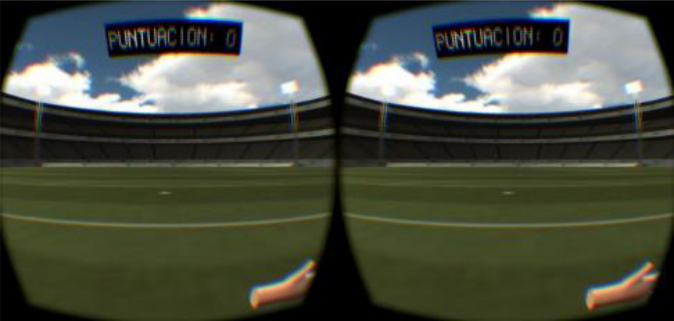
\includegraphics[scale=0.5]{img/eiah_baldominos.png}
    \end{frame}
    
    \begin{frame}{\secname}
        Toussaint : Manipulation d'un trocard, en combinant les données d'un bras haptique et du retour de force associé et d'un occulomètre (pour suivre la trajectoire du regard). \mycite{BMT_2015}\\
        \centering
        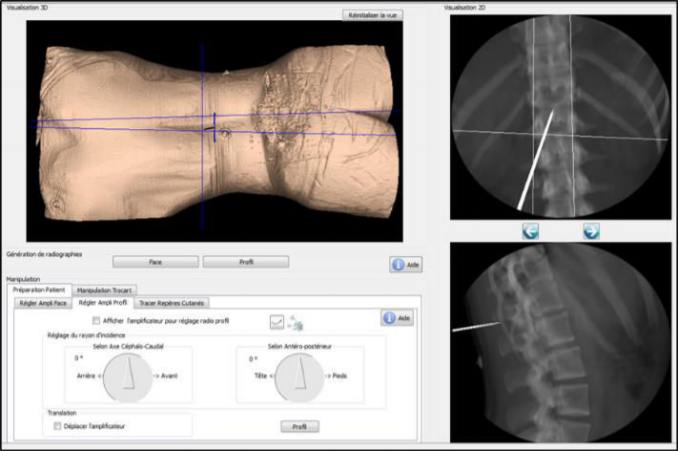
\includegraphics[scale=0.4]{img/eiah_toussaint.png}
    \end{frame}
    
    \begin{frame}{\secname}
         Gameiro \textit{et al.} : Ludification de l'apprentissage de la langue des signes \mycite{Gameiro2014KST}\\
        \centering
        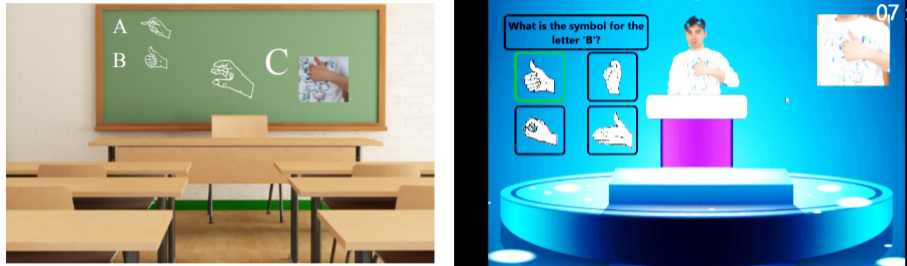
\includegraphics[scale=0.4]{img/eiah_gameiro.png}
    \end{frame}
    
    \begin{frame}{\secname}
         Xu \textit{et al.} : Apprentissages de gestes variés (manipuler un métier à tisser, tirer à l’arc, chevaucher un cheval, manipuler des panneaux) à l'aide de l'adaptation du parcours d'apprentissage \mycite{Xu2019Ptt}\\
        \centering
        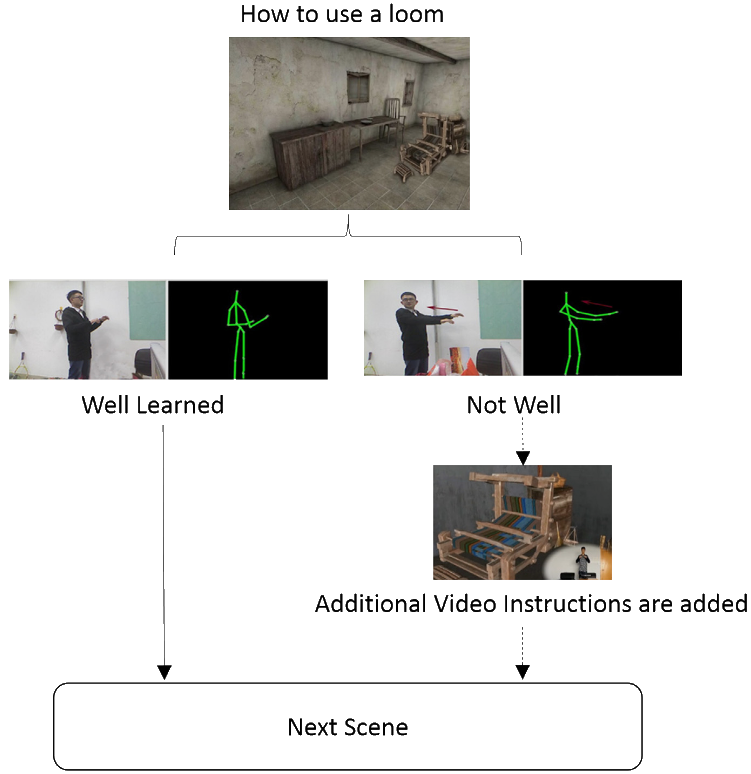
\includegraphics[scale=0.3]{img/eiah_xu.png}
    \end{frame}
    
    \begin{frame}{\secname}
         Morel : évaluation de gestes sportifs à l'aide de séries temporelles. Les mouvements de l'apprenant et de l'expert sont recalés spatialement et temporellement, puis les erreurs sont calculés et affichées \mycite{Morel2017Mts}\\
        \centering
        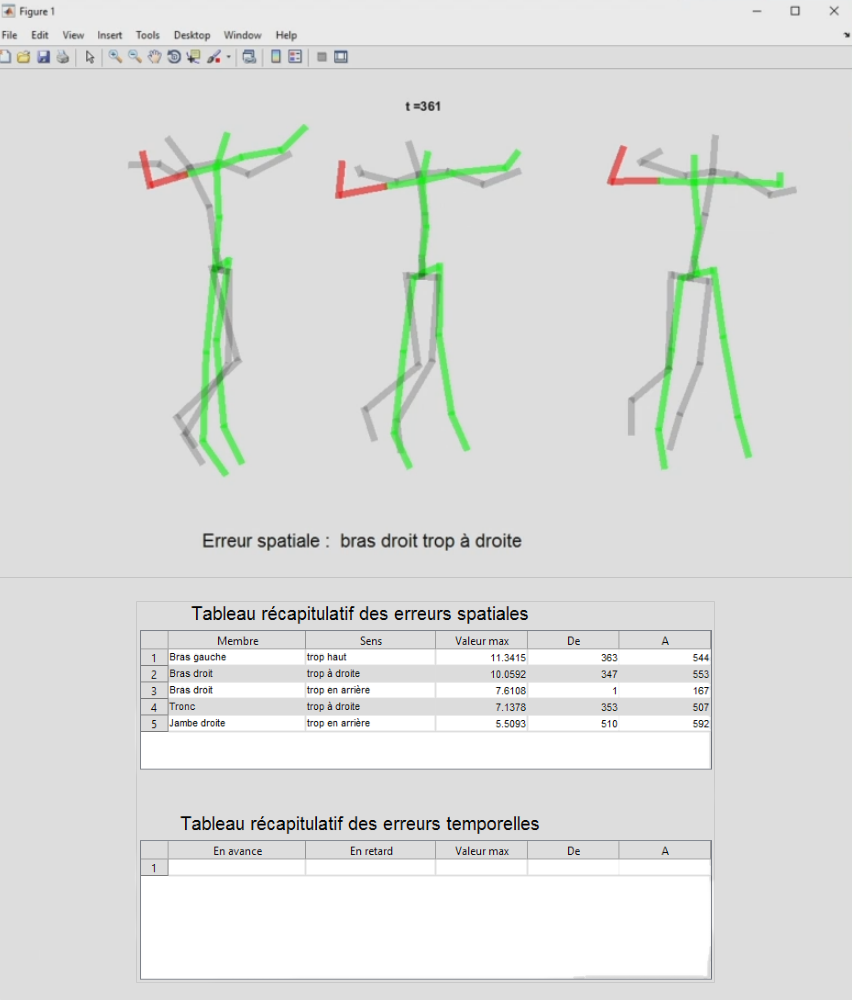
\includegraphics[scale=0.25]{img/eiah_morel.png}
    \end{frame}
    
    
    \begin{frame}{\secname}
        Plusieurs limites récurrentes :
        \begin{itemize}[label=$\bullet$]
            \item Ré-ingénierie nécessaire pour utiliser l'EIAH dans d'autres domaines
            \item Dans le cas d'apprentissage supervisé, nécessite une base de donnée d'apprentissage étiquetée conséquente, la reconstitution d'un corps pour l'utilisation dans un autre domaine et la connaissance précise des classes \textit{a priori}
            \item Dans les systèmes automatiques (s'affranchissant de l'expert), les retours peuvent manquer de sémantique, et les retours peuvent être difficile à interpréter pour des non-experts
        \end{itemize}
    \end{frame} 
    
    \begin{frame}{\subsecname}
        \begin{block}{Domaine médical}
            \begin{itemize}[label=$\bullet$]
                \item Rééducation
                \item Visualisation de la démarche du patient à distance (analyse de la démarche \mycite{Chen2016TPG})
                \item Entraînement de plusieurs chirurgiens dans un environnement virtuel (chirurgie \mycite{Pulijala2017VRS}), etc.
            \end{itemize}
        \end{block}
    \end{frame}
    
    \begin{frame}{\subsecname}
        \begin{block}{Sport}
            \begin{itemize}[label=$\bullet$]
                \item Analyse des vidéos de l'apprenant avant et après l'entrainement (visualisation puis reproduction du mouvement de l'expert en karaté, \mycite{Burns2011Uvh})
                \item Superposition du modèle de l'apprenant et de l'expert pour la reproduction et l'apprentissage (lancer au football américain, \mycite{LeNaour2019S3V})
                \item Projection du modèle de l'apprenant sur celui de l'expert en temps réel (golf, \mycite{Kora20151559})
                \item Superposition de l'apprenant à un ou des modèles experts, en fonction (archerie japonaise, \mycite{Yoshinaga2015Doa})
            \end{itemize}
        \end{block}
    \end{frame}
    
    \subsection{Analyse par observation d'indicateurs}
    \begin{frame}{\subsecname}
        \begin{block}{Domaine médical}
            \begin{itemize}[label=$\bullet$]
                \item Comparaison de la trajectoire d'un objet par rapport à une trajectoire de référence (forceps \mycite{Pham2010Tdg}, porte-aiguille \mycite{Despinoy2016UTS})
                \item Analyse de l'évolution de la maladie de Parkison, à l'aide de la distance réalisée à chaque pas, balancement de la posture, degré de balancement des bras et constance de l'intervalle de temps entre deux pas \mycite{Wang2013HMM}
            \end{itemize}
        \end{block}
    \end{frame}
    
    \begin{frame}{\subsecname}
        \begin{block}{Sport}
            \begin{itemize}[label=$\bullet$]
                \item Analyse basée sur les positions relatives des parties du corps à des moments clés du lancer (lancer de disque, \mycite{Yamaoka2013FoF})
                \item alignement spatial d'un membre par rapport au membre de référence, et différence entre les chemins de déformations induits par les alignements des membres de l’apprenant et de l’expert \mycite{Morel2017Mts}
                \item Trajectoire et vitesse du poignet (service au tennis, \mycite{Makio2007DoS})
            \end{itemize}
        \end{block}
    \end{frame}
    
    \begin{frame}{\subsecname}
        \begin{block}{Arts}
            \begin{itemize}[label=$\bullet$]
                \item Analyse de la correlation spatiale et temporelle entre le modèle de l'apprenant et de l'expert (danse \mycite{Maes2012DtM})           
                \item Décomposition du mouvement à l'aide d'un seul descripteur projeté dans un espace sphérique, puis comparaison à une base de données de mouvements de danse (danse \mycite{Kyan2015ABD})
                \item Détermination du mode jeu à l'aide d'informations cinétiques du mouvement : vitesse, tremblement, impulsion (violon \mycite{Rasamimanana2008EbA})
            \end{itemize}
        \end{block}
    \end{frame}
    
    \subsection{Analyse par détection de séquence ordonnée d'actions}
    \begin{frame}{\subsecname}
        \begin{block}{Environnements virtuels}
            \begin{itemize}[label=$\bullet$]
                \item Description du scénario pédagogique par l'expert, à l'aide d'une association activité / séquence d'actions, elles-mêmes divisées en séquences de comportement élémentaires : observation, déplacement, interaction, communication \mycite{Mahdi2019TaE}       
                \item Proposition d'un parcours à réaliser par l'expert, personnalisable à l'aide de points de contrôle à passer dans un ordre précis, puis détection de la présence d'un objet ou du corps de l'apprenant au sein de ces zones pour segmenter le mouvement. Enfin, chaque segment est comparé à la référence de l'expert \mycite{Delest2019MaE}
            \end{itemize}
        \end{block}
    \end{frame}
    
    \subsection{Analyse basée sur des techniques d'apprentissage automatique}
    \begin{frame}{\subsecname}
        \begin{block}{Analyse automatique}
            \begin{itemize}[label=$\bullet$]
                \item Évaluation de gestes sans \textit{a priori} sur le geste en lui-même, afin de déterminer les règles sous-jacentes à l'évaluation subjective des experts (patinage artistique et plongeon olympiques \mycite{Pirsiavash2014AQA})
                \item Segmentation, reconnaissance et évaluation de gestes à l'aide d'algorithmes de logique floue. Extraction de descripteurs cinétiques, reconnaissance à l'aide de classifieurs binaires pré-entrainés, puis évaluation par rapport aux mouvements contenus dans une base de données (gestes divers \mycite{Patrona2018MaA})
            \end{itemize}
        \end{block}
    \end{frame}
    
    \subsection{Bilan des systèmes existants}
    \begin{frame}{\subsecname}
        \begin{block}{Systèmes basés sur l'analyse humaine}
            \begin{itemize}[label=$\bullet$]
                \item Utilisateurs finaux au centre du système
                \item Savoir de l'expert parfois indispensable et non aisément formalisable (domaine médical)
                \item Parfois pas utilisables par un non-expert (nécessité de combiner les retours du système à une expertise scientifique)
                \item Possibilité de proposer des visualisations du mouvement de l'expert et de l'apprenant, facilement utilisables par un non-expert et génériques, mais ne proposent pas d'analyse
            \end{itemize}
        \end{block}
        
        \begin{block}{Systèmes utilisant des descripteurs}
            \begin{itemize}[label=$\bullet$]
                \item Fournissent un ensemble de valeur permettant d'assister l'expert dans son jugement
                \item Nécessiter de posséder des connaissances scientifiques pour l'interprétation des valeurs
                \item Souvent fortement couplés au domaine applicatif choisi, ainsi qu'au matériel utilisé
            \end{itemize}
        \end{block}
    \end{frame}
    
    \begin{frame}{\subsecname}
        \begin{block}{Systèmes d'analyse automatique}
            \begin{itemize}[label=$\bullet$]
                \item Permettent de s'affranchir de l'expert une fois le système conçu
                \item Retours parfois peu exhaustif (score seulement, sans indication sur les parties du corps qui ne font pas correctement le geste)
                \item Manque d'indications sur comment corriger le geste
                \item L'absence d'expert lors de l'utilisation limite l'exhaustivité des retours
                \item Généricité au regard du domaine considéré souvent faible
            \end{itemize}
        \end{block}
        
        \begin{block}{Systèmes basés sur la détection d'actions}
            \begin{itemize}[label=$\bullet$]
                \item Cherchent à segmenter le mouvement en unités élémentaires, puis proposent une comparaison de l'ordre de ces unités élémentaires
                \item Intégration de la connaissance experte dès la conception, manque de généricité
                \item Certains systèmes introduisent la réutilisabilité dès leur conception \mycite{Mahdi2019TaE, Delest2019MaE}
            \end{itemize}
        \end{block}
        
        \begin{block}{Systèmes basés sur l'apprentissage automatique}
            \begin{itemize}[label=$\bullet$]
                \item Intégration de la connaissance experte \textit{a priori}
                \item Nécessitent une base de données (d'apprentissage et de comparaison) volumineuse et spécialisée
            \end{itemize}
        \end{block}
    \end{frame}
    
    \begin{frame}{\subsecname}
        \begin{block}{Sport}
            \begin{itemize}[label=$\bullet$]
                \item Analyse des vidéos de l'apprenant avant et après l'entrainement (visualisation puis reproduction du mouvement de l'expert en karaté, \mycite{Burns2011Uvh})
                \item Superposition du modèle de l'apprenant et de l'expert pour la reproduction et l'apprentissage (lancer au football américain, \mycite{LeNaour2019S3V})
                \item Projection du modèle de l'apprenant sur celui de l'expert en temps réel (golf, \mycite{Kora20151559})
                
            \end{itemize}
        \end{block}
    \end{frame}
    
    \section{Descripteurs du mouvement} 
    
    \begin{frame}{\subsecname}
        Plusieurs classifications de descripteurs existent :
        \begin{itemize}[label=$\bullet$]
            \item Laban Movement Analysis (LBA)
            \item HBF49 \mycite{Delaye2013HBF}, HIF3D \mycite{Boulahia2016HIF}
            \item 
        \end{itemize}
        
        \centering
        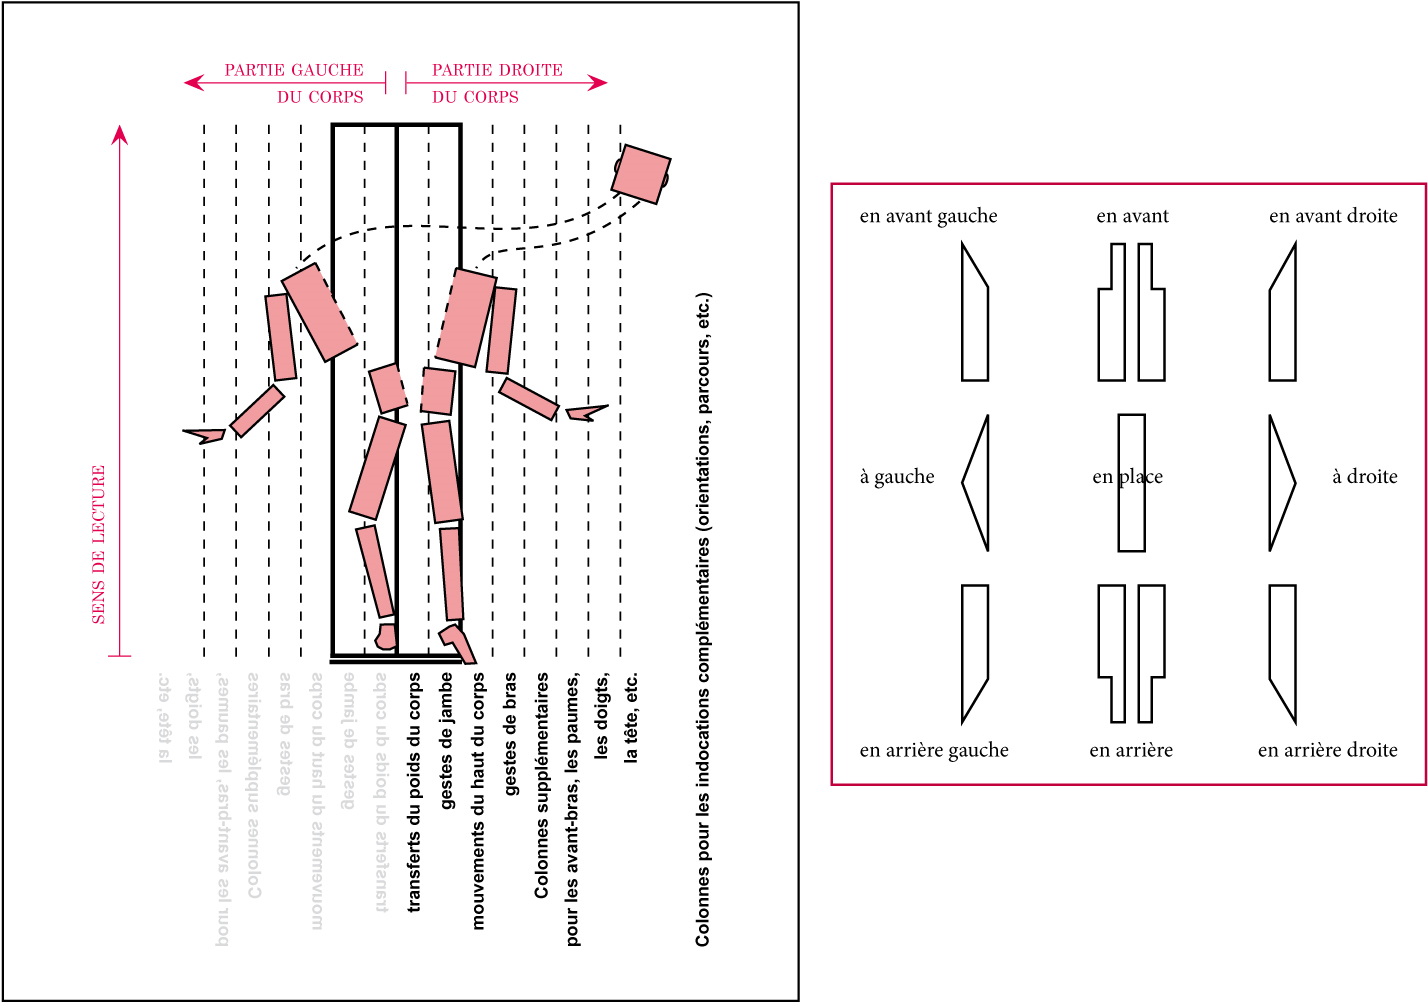
\includegraphics[scale=0.15]{img/laban_2.png}
    \end{frame}
    
    \begin{frame}{\subsecname}
        \begin{itemize}[label=$\bullet$]
            \item Larboulette et Gibet : classification en descripteurs bas-niveau (quantités cinématiques, dynamiques ou géométrique) / haut-niveau (quantités exploitables dans une évaluation visuelle du mouvement ou par un expert), cinématique / géométrique, corps / environnement \mycite{larboulette2015Descriptors}
            \item Morel : classification en trois grandes familles, descripteurs reposant sur un modèle du corps humain, holistiques (dynamique globale de l'objet considéré) et descripteurs locaux (à partir de points d'intérêt isolés) \mycite{Morel2017Mts}
        \end{itemize}
    \end{frame}
    
    \begin{frame}{\subsecname}
        Ensembles de descripteurs pour l'indexation et la recherche de mouvement :
        \begin{itemize}[label=$\bullet$]
            \item Sakurai \textit{et al.} : plusieurs aires extraites d'un pentagone calculé, puis utilisation de la DTW pour la recherche \mycite{Sakurai2015Ros}
            \item Xiao \textit{et al.} : projection du mouvement 3D sur 8 plans 2D, puis réduction à l'aide d'un algorithme de séléction de caractéristiques semi-supervisé \mycite{Xiao2015Sbh}
        \end{itemize}
    \end{frame}
    
    \begin{frame}{\subsecname}
        Ensembles de descripteurs pour la reconnaissance d'actions :
        \begin{itemize}[label=$\bullet$]
            \item  Delaye et Anquetil : descripteurs servant à caractériser les mouvements d'écriture : points de début et de fin de trait, angles formés par les différentes parties des lettres, proportion de trajectoires dirigées, etc. (HBF49) \mycite{Delaye2013HBF}
            \item Boulahia \textit{et al.} : généralisation de HBF49 à une trajectoire 3D (HIF3D) \mycite{Boulahia2016HIF}
            \item Rao \textit{et al.} : caractérise les moments d'inflexion dans la trajectoire, afin de les segmenter en unités élémentaires \mycite{Rao2002VRR}
        \end{itemize}
    \end{frame}
    
    \begin{frame}{\subsecname}
        \begin{itemize}[label=$\bullet$]
            \item Réutisabilité non assurée
            \item Utilisation dans un contexte d'apprentissage non considérée
            \item Compréhension et utilisation par un humain non assurées
            \item Redondance sémantique
        \end{itemize}
    \end{frame}
    
    \begin{block}{Systèmes basés sur l'analyse humaine}
            \begin{itemize}[label=$\bullet$]
                \item Utilisateurs finaux au centre du système
                \item Savoir de l'expert parfois indispensable et non aisément formalisable (domaine médical)
                \item Parfois pas utilisables par un non-expert (nécessité de combiner les retours du système à une expertise scientifique)
                \item Possibilité de proposer des visualisations du mouvement de l'expert et de l'apprenant, facilement utilisables par un non-expert et génériques, mais ne proposent pas d'analyse
            \end{itemize}
        \end{block}
        
        \begin{block}{Systèmes utilisant des descripteurs}
            \begin{itemize}[label=$\bullet$]
                \item Fournissent un ensemble de valeur permettant d'assister l'expert dans son jugement
                \item Nécessiter de posséder des connaissances scientifiques pour l'interprétation des valeurs
                \item Souvent fortement couplés au domaine applicatif choisi, ainsi qu'au matériel utilisé
            \end{itemize}
        \end{block}
    \end{frame}
    
    \begin{frame}{\subsecname}
        \begin{block}{Systèmes d'analyse automatique}
            \begin{itemize}[label=$\bullet$]
                \item Permettent de s'affranchir de l'expert une fois le système conçu
                \item Retours parfois peu exhaustif (score seulement, sans indication sur les parties du corps qui ne font pas correctement le geste)
                \item Manque d'indications sur comment corriger le geste
                \item L'absence d'expert lors de l'utilisation limite l'exhaustivité des retours
                \item Généricité au regard du domaine considéré souvent faible
            \end{itemize}
        \end{block}
        
        \begin{block}{Systèmes basés sur la détection d'actions}
            \begin{itemize}[label=$\bullet$]
                \item Cherchent à segmenter le mouvement en unités élémentaires, puis proposent une comparaison de l'ordre de ces unités élémentaires
                \item Intégration de la connaissance experte dès la conception, manque de généricité
                \item Certains systèmes introduisent la réutilisabilité dès leur conception \mycite{Mahdi2019TaE, Delest2019MaE}
            \end{itemize}
        \end{block}
        
        \begin{block}{Systèmes basés sur l'apprentissage automatique}
            \begin{itemize}[label=$\bullet$]
                \item Intégration de la connaissance experte \textit{a priori}
                \item Nécessitent une base de données (d'apprentissage et de comparaison) volumineuse et spécialisée
            \end{itemize}
        \end{block}
    
    \subsection{Classifications en descripteurs élémentaires}
    \begin{frame}{\subsecname}
    Proposition de classification en descripteurs élémentaires
        \begin{itemize}[label=$\bullet$]
            \item Descripteurs non issus de calculs, de ré-interprétations ou d'ensembles de descripteurs « bas-niveau » du mouvement
            \item Répondent à des besoins d'observation et d'analyse
        \end{itemize}
    \end{frame}
    
    \subsection{Incohérence des positions}
    \begin{frame}{Incohérence des positions successives}
    \centering
        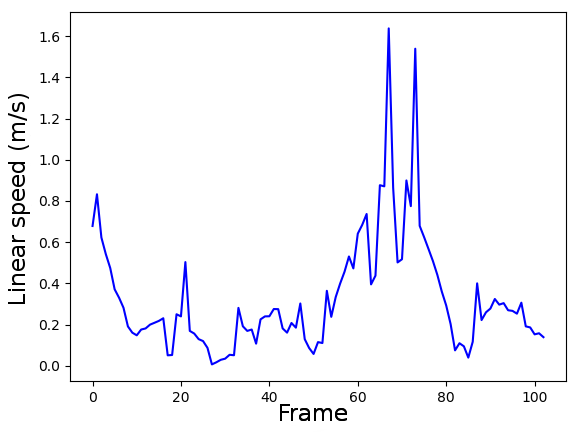
\includegraphics[scale=0.7]{img/linear_speed_artifacts.png}
    \end{frame}
    
    \begin{frame}{Incohérence des positions successives}
    Plusieurs hypothèses :
        \begin{center}
                \begin{table}[h!]
                \resizebox{\linewidth}{!}{%
                \begin{tabular}{l|l|l}
                    & \makecell{Interpolation} & Pas d'interpolation \\\hline
                    \makecell{Intervalle de temps\\constant} & \makecell{Mauvaise interpolation} & \textit{Frames} manquantes                  \\\hline
                    \makecell{Intervalle de temps\\non-constant} & \makecell{Mauvaise posture\\dû a un indice temporel erroné} & \makecell{\textit{Frames} affichées\\au mauvais moment}
                \end{tabular}}
                \end{table}
        \end{center}
    \end{frame}
    
    \begin{frame}{Retour donné à l'expert}
        \centering
            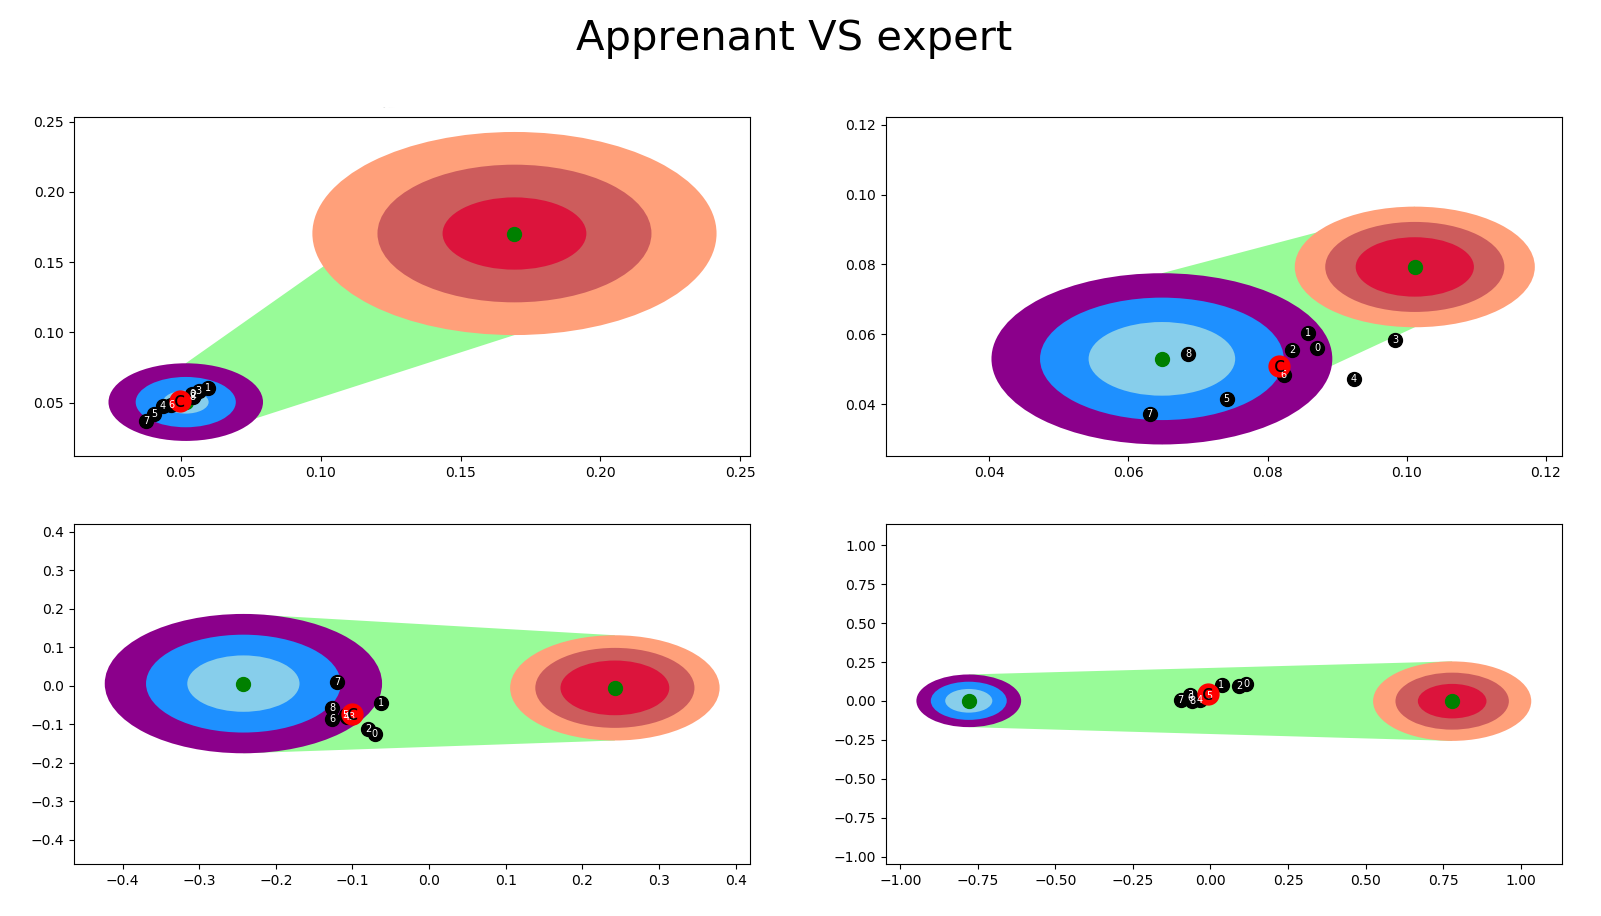
\includegraphics[scale=0.25]{img/feedback_grp_example.png}
    \end{frame}
    
    \subsection{Données utilisées}  
    \begin{frame}{\secname : \subsecname}
        \begin{block}{Descripteurs}
            \begin{itemize}
                \item la norme du vecteur vitesse (SN)
                \item la norme du vecteur vitesse en X, Y, Z (S x/y/z)
                \item la direction du vecteur vitesse en X, Y, Z (Sd x/y/z)
                \item la norme du vecteur vitesse ainsi que la direction de ce vecteur en X, Y, Z (SNDxyz)
            \end{itemize}
        \end{block}
        
        \begin{block}{Articulations}
            \begin{itemize}
                \item la main
                \item l'avant-bras
                \item le bras
                \item l'épaule
            \end{itemize}
        \end{block}
    \end{frame}

    \begin{frame}{\secname}
        \begin{itemize}[label=$\bullet$]
            \item Explication des données non-alignées
            \item Création de nouveaux descripteurs à l'aide d'un système fondé sur des patrons de conception
            \item Expérimentation à plus grande échelle
            \item Expérimentation dans d'autres domaines applicatifs
            \item Expérimentation d'apprentissage en autonomie
            \item Clustering récursif
        \end{itemize}
    \end{frame}

    \subsubsection{Schéma de l'installation}
    \begin{frame}{\subsecname : \subsubsecname}
        \centering
        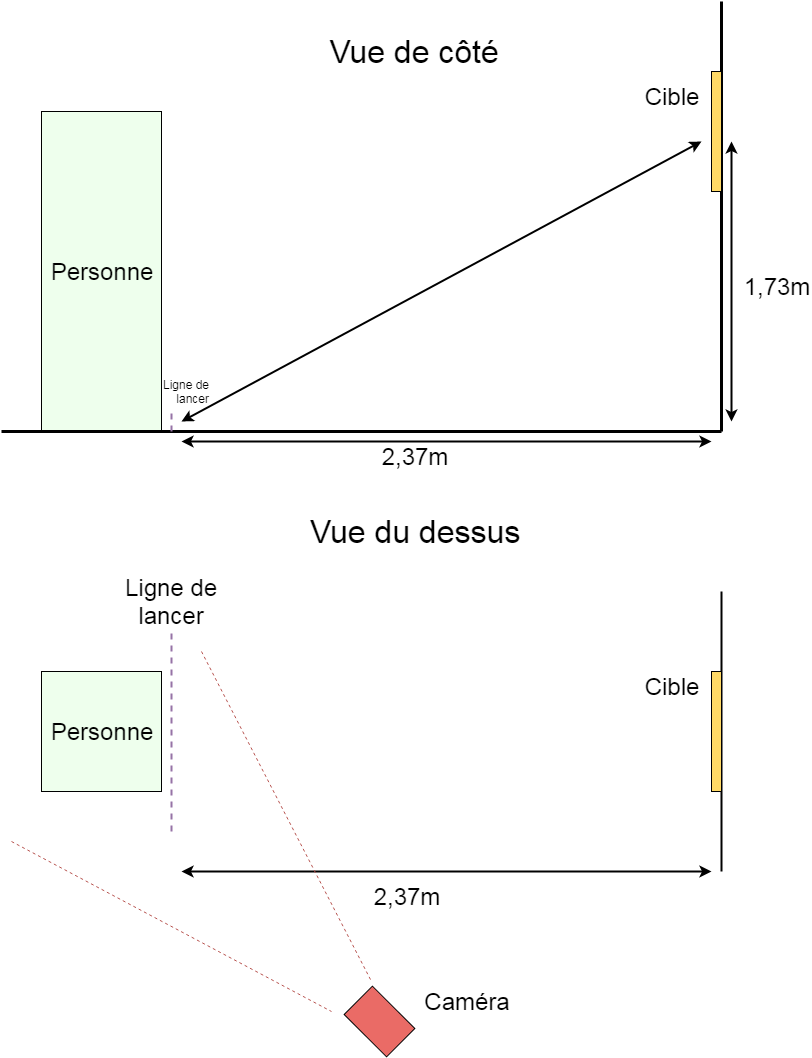
\includegraphics[scale=0.2]{img/Darts_scheme.png}
    \end{frame}
\if